% Provenance (never printed): see sources/outline_sources.md (Year 3:
% atmospheric dynamics: vorticity and potential vorticity, Rossby waves,
% baroclinic instability, the general circulation and the Hadley cell).
% Brief: sources/book5/BRIEFS.md, ch. 20. Curves from
% figdata/bachelor-3/rossby_waves.py, eady.py and held_hou.py. Exercise and
% problem values in the Book 5 scratch calculator calc/ch20.py. The waves,
% shears and parcels of the exercises and the problem are invented.
\chapter{Atmosferische dynamica}\label{ch:b3:atmospheric-dynamics}

Op een winterkaart van de bovenste troposfeer cirkelt de straalstroom niet als een
gladde ring om de pool. Hij meandert in een paar grote golven rond het
halfrond, met dalen die naar de subtropen reiken en kammen naar de
pool, en aan het oppervlak ontstaan depressies die enkele dagen groeien en
daarna eronder weer sterven. De golven verplaatsen zich langzaam, soms tegen de wind in die
ze meevoert. Hun aantal, hun snelheid en de groei van de stormen eronder
volgen uit één behouden grootheid, de vorticiteit van de lucht, vanuit
de ruimte bekeken, en uit de energie opgeslagen in het temperatuurcontrast tussen de
tropen en de polen.

\begin{recall}
Vorticiteit en circulatie komen in de natuurkundeboeken voor. De Rossby-golven van de
bovenste troposfeer, dalen en kammen, de extratropische cycloon en het
principe van numerieke weersverwachting worden beschreven in Boek~4,
in het hoofdstuk over weersystemen. De Hadley-, Ferrel- en poolcellen, de
straalstromen, de westenwinden en de wind door impulsmoment van een ring lucht
staan in Boek~3, in het hoofdstuk over de algemene circulatie van de
atmosfeer, en het poolwaartse warmtetransport in het hoofdstuk over
straling en warmtetransport. De Coriolisparameter $f$, het $\beta$-vlak,
de Rossby-straal en de \omterm{thm:b3:gfd-foundations:thermal-wind}{thermische wind} staan in
Hoofdstuk~\ref{ch:b3:gfd-foundations}.
\end{recall}

\section{Vorticiteit}\label{sec:b3:atmospheric-dynamics:vorticity}

De vorticiteit van een vloeistof, de rotatie van haar snelheid, is twee keer haar lokale
hoeksnelheid. Voor de grootschalige atmosfeer telt alleen de verticale
component, en de rotatie van de Aarde draagt daaraan bij.

\begin{definition}[Relatieve, planetaire en absolute vorticiteit]\label{def:b3:atmospheric-dynamics:vorticity-kinds}
Voor een horizontale snelheid $(u, v)$ is de \emph{relatieve
vorticiteit}\index{relatieve vorticiteit} de verticale component van de rotatie
van de snelheid ten opzichte van de grond, $\zeta = \partial v/\partial x -
\partial u/\partial y$, positief bij rotatie tegen de klok in, van bovenaf gezien.
De \emph{planetaire vorticiteit}\index{planetaire vorticiteit} is de verticale
component van de vorticiteit van de rotatie van de Aarde, $2\Omega\sin\varphi =
f$. De \emph{absolute vorticiteit}\index{absolute vorticiteit} is hun som,
$\zeta + f$.
\end{definition}

Op het Noordelijk Halfrond is een depressie, waar de lucht tegen de klok in draait,
heeft $\zeta > 0$ en heet cyclonaal; een anticycloon heeft $\zeta < 0$. Een
wind van \qty{15}{m/s} die op een cirkel van \qty{1000}{km} draait heeft $\zeta =
2V/R = \qty{3e-5}{s^{-1}}$ bij starre rotatie, een derde van $f$ op \ang{45}:
het planetaire deel is meestal het grootste.

\begin{theorem}[Barotrope vorticiteitsvergelijking]\label{thm:b3:atmospheric-dynamics:bve}
In een wrijvingsloze, tweedimensionale stroming zonder horizontale divergentie op een
$\beta$-vlak wordt de \omterm{def:b3:atmospheric-dynamics:vorticity-kinds}{absolute vorticiteit} van elk luchtpakketje behouden:
\[
\frac{\mathrm D(\zeta + f)}{\mathrm Dt} = 0 ,
\qquad\text{dat wil zeggen}\qquad
\frac{\partial\zeta}{\partial t} + u\frac{\partial\zeta}{\partial x} + v\frac{\partial\zeta}{\partial y} + \beta v = 0 .
\]
Dit is de \emph{barotrope vorticiteitsvergelijking}\index{barotrope vorticiteitsvergelijking}.
\end{theorem}

\begin{proof}
De horizontale impulsvergelijkingen zijn $\mathrm Du/\mathrm Dt - fv =
-(1/\rho_0)\partial p/\partial x$ en $\mathrm Dv/\mathrm Dt + fu =
-(1/\rho_0)\partial p/\partial y$. Differentieer de tweede naar
$x$, de eerste naar $y$, en trek af: de druk valt weg.
Met $\delta = \partial u/\partial x + \partial v/\partial y$ leveren de
advectietermen $\partial_x(u\,\partial_xv + v\,\partial_yv) -
\partial_y(u\,\partial_xu + v\,\partial_yu) = u\,\partial_x\zeta +
v\,\partial_y\zeta + \zeta\delta$, en de Coriolistermen $f\delta + \beta
v$. Dus $\mathrm D\zeta/\mathrm Dt + \beta v = -(\zeta + f)\,\delta$. Voor
$\delta = 0$, en omdat $\mathrm Df/\mathrm Dt = \beta v$, $\mathrm D(\zeta +
f)/\mathrm Dt = 0$.
\end{proof}

Het bewijs leverde ook de algemene wet op, $\mathrm D(\zeta + f)/\mathrm Dt =
-(\zeta + f)\delta$: convergentie laat een kolom sneller draaien, divergentie vertraagt hem,
net als een schaatsster die de armen intrekt of spreidt. In een laag waarvan
de diepte verandert, is convergentie gekoppeld aan het uitrekken van de kolom, en
wordt de behouden grootheid een verhouding.

\begin{definition}[Potentiële vorticiteit]\label{def:b3:atmospheric-dynamics:pv}
De \emph{potentiële vorticiteit}\index{potentiële vorticiteit} van een kolom van een
homogene laag met diepte $h$ is $q = (\zeta + f)/h$. In een continu gelaagde
vloeistof is de potentiële vorticiteit van Ertel $q = (\vec\omega_a\cdot
\nabla\theta)/\rho$, met $\vec\omega_a$ de absolute vorticiteitsvector en
$\theta$ de potentiële temperatuur.
\end{definition}

\begin{theorem}[Behoud van potentiële vorticiteit]\label{thm:b3:atmospheric-dynamics:pv}
In een homogene, hydrostatische, wrijvingsloze laag met variabele diepte $h$ waarvan
de horizontale snelheid niet met de hoogte varieert, $\mathrm Dq/\mathrm Dt = 0$
voor $q = (\zeta + f)/h$.
\end{theorem}

\begin{proof}
Uit het bewijs hierboven volgt $\mathrm D(\zeta + f)/\mathrm Dt = -(\zeta + f)\delta$.
Massabehoud in een kolom van uniforme dichtheid geeft $\mathrm Dh/\mathrm
Dt = -h\delta$. Dan volgt $\mathrm Dq/\mathrm Dt = (1/h)\,\mathrm D(\zeta +
f)/\mathrm Dt - ((\zeta + f)/h^2)\,\mathrm Dh/\mathrm Dt = -(\zeta +
f)\delta/h + (\zeta + f)\delta/h = 0$.
\end{proof}

De vorm van Ertel blijft op dezelfde manier behouden bij een adiabatische, wrijvingsloze
stroming van een gelaagde vloeistof, waarbij de afstand tussen twee oppervlakken van
constante $\theta$ de rol van $h$ speelt. Een luchtkolom die een
bergketen oversteekt, wordt onderweg omhoog samengedrukt: haar \omterm{def:b3:atmospheric-dynamics:vorticity-kinds}{absolute vorticiteit} daalt, ze
draait anticyclonaal over de kam, en ze rekt zich uit en draait
cyclonaal aan de lijzijde. Behoud van
absolute of \omterm{def:b3:atmospheric-dynamics:pv}{potentiële vorticiteit} is het herstellende mechanisme van de golven
van de volgende paragraaf, zoals de figuur hieronder toont.

\begin{omfigure}
\begin{tikzpicture}[>=stealth, font=\small, declare function={w(\x)=0.9*sin(\x r);}]
\draw[black!40, dashed] (0,0) -- (12.6,0) node[right, font=\scriptsize] {breedtegraad $\varphi_0$};
\draw[thick, omDef, domain=0:12.566, samples=120] plot (\x, {w(\x)});
\foreach \x in {0.785, 2.356, 3.927, 5.498, 7.069, 8.639, 10.21, 11.78}
  \fill (\x, {w(\x)}) circle (0.06);
% crests: clockwise (anticyclonic), troughs: anticlockwise (cyclonic)
\foreach \x in {1.571, 7.854} {
  \draw[->, omThm, thick] (\x+0.45,{w(\x)+0.05}) arc (0:-300:0.45);
  \node[font=\scriptsize, omThm] at (\x,{w(\x)+0.75}) {$\zeta < 0$};}
\foreach \x in {4.712, 10.996} {
  \draw[->, omMeth, thick] (\x+0.45,{w(\x)-0.05}) arc (0:300:0.45);
  \node[font=\scriptsize, omMeth] at (\x,{w(\x)-0.75}) {$\zeta > 0$};}
\foreach \x in {3.1416, 9.4248} \draw[->, very thick] (\x,0.45) -- (\x,-0.45);
\foreach \x in {6.2832} \draw[->, very thick] (\x,-0.45) -- (\x,0.45);
\draw[->, thick] (8.4,-2.25) -- (6.4,-2.25) node[left, font=\scriptsize] {het patroon beweegt naar het westen};
\draw[->] (0,-2.25) -- (1.4,-2.25) node[right, font=\scriptsize] {oost};
\draw[->] (0,-2.25) -- (0,-1.65) node[above, font=\scriptsize] {noord};
\end{tikzpicture}

\par\smallskip{\small Hoe een Rossby-golf beweegt (schematisch, noordelijk
halfrond). Een keten van pakketjes in rust op breedtegraad $\varphi_0$ wordt
uit zijn evenwicht gebracht tot een golf. Met behoud van $\zeta + f$ krijgen de naar het noorden verplaatste pakketjes, waar
$f$ groter is, een met de klok mee gerichte \omterm{def:b3:atmospheric-dynamics:vorticity-kinds}{relatieve vorticiteit}; de naar het zuiden verplaatste krijgen
een tegen de klok in gerichte. Tussen een kam en de trog ten oosten ervan is de geïnduceerde stroming
naar het zuiden gericht, tussen een trog en de kam ten oosten ervan naar het noorden (zwarte
pijlen): de verplaatsing groeit ten westen van elke kam, en het hele patroon
schuift naar het westen op.}\label{fig:b3:atmospheric-dynamics:restoring}
\end{omfigure}

\section{Rossby-golven}\label{sec:b3:atmospheric-dynamics:rossby}

Boek~4 beschreef de Rossby-golven van de bovenste troposfeer. De
\omterm{thm:b3:atmospheric-dynamics:bve}{barotrope vorticiteitsvergelijking} verklaart ze. Men schrijft de stroming als een uniforme
westenwind $U$ plus een kleine storing met stroomfunctie $\psi'$, zodat
$u' = -\partial\psi'/\partial y$, $v' = \partial\psi'/\partial x$ en $\zeta'
= \nabla^2\psi'$.

\begin{theorem}[Dispersie van Rossby-golven]\label{thm:b3:atmospheric-dynamics:rossby}
Kleine storingen $\psi' \propto \mathrm e^{\mathrm i(kx + ly - \omega t)}$
van een uniforme westenwind $U$ op een $\beta$-vlak voldoen aan de
\emph{dispersierelatie van Rossby-golven}\index{dispersierelatie van Rossby-golven}
\[
\omega = Uk - \frac{\beta k}{k^2 + l^2} .
\]
Hun oostwaartse fasesnelheid is $c = \omega/k = U - \beta/K^2$, met $K^2 =
k^2 + l^2$, en hun oostwaartse groepssnelheid $c_g = \partial\omega/\partial
k = U + \beta(k^2 - l^2)/K^4$.
\end{theorem}

\begin{proof}
Gelineariseerd rond $U$ luidt de \omterm{thm:b3:atmospheric-dynamics:bve}{barotrope vorticiteitsvergelijking}
$(\partial_t + U\partial_x)\nabla^2\psi' + \beta\,\partial_x\psi' = 0$, de
producten van kleine grootheden vallen weg en $\zeta$ van de basisstroming
is nul. Voor de vlakke golf geldt $\partial_t \to -\mathrm i\omega$,
$\partial_x \to \mathrm ik$ en $\nabla^2 \to -K^2$: $(-\mathrm i\omega +
\mathrm iUk)(-K^2) + \mathrm i\beta k = 0$, dat is $(\omega - Uk)K^2 =
-\beta k$. Differentiëren van $\omega$ naar $k$ geeft $c_g = U -
\beta/K^2 + 2\beta k^2/K^4$, wat de opgegeven vorm is.
\end{proof}

\begin{omfigure}
\begin{tikzpicture}
\begin{groupplot}[group style={group size=2 by 1, horizontal sep=1.7cm},
  width=0.48\linewidth, height=0.46\linewidth, tick label style={font=\scriptsize},
  label style={font=\small}, legend style={font=\scriptsize, draw=none, fill=none}]
\nextgroupplot[xlabel={zonaal golfgetal $n$}, ylabel={snelheid (\unit{m/s})},
  xmin=1, xmax=12, ymin=-40, ymax=60, legend pos=north east, legend cell align=left,
  title={\small \ang{45} NB}]
% computed in figdata/bachelor-3/rossby_waves.py
\addplot[omThm, thick] table[x=n, y=c15] {figdata/out/bachelor-3-rossby_waves-disp.dat};
\addlegendentry{$c$, $U = 15$}
\addplot[omThm, thick, densely dashed] table[x=n, y=cg15] {figdata/out/bachelor-3-rossby_waves-disp.dat};
\addlegendentry{$c_g$, $U = 15$}
\addplot[omDef, thick] table[x=n, y=c0] {figdata/out/bachelor-3-rossby_waves-disp.dat};
\addlegendentry{$c$, $U = 0$}
\addplot[omDef, thick, densely dashed] table[x=n, y=cg0] {figdata/out/bachelor-3-rossby_waves-disp.dat};
\addlegendentry{$c_g$, $U = 0$}
\addplot[black!50, thin, domain=1:12, samples=2, forget plot] {0};
\nextgroupplot[xlabel={breedtegraad (\unit{\degree} NB)}, ylabel={stationair golfgetal $n_s$},
  xmin=20, xmax=75, ymin=0, ymax=9, legend pos=north east, legend cell align=left]
\addplot[omMeth, thick] table[x=lat, y=n10] {figdata/out/bachelor-3-rossby_waves-stat.dat};
\addplot[omDef, thick] table[x=lat, y=n15] {figdata/out/bachelor-3-rossby_waves-stat.dat};
\addplot[omThm, thick] table[x=lat, y=n20] {figdata/out/bachelor-3-rossby_waves-stat.dat};
\addplot[black, only marks, mark=*, mark size=1.1pt] table[x=lat, y=ns] {figdata/out/bachelor-3-rossby_waves-statobs.dat};
\legend{\qty{10}{m/s}, \qty{15}{m/s}, \qty{20}{m/s}, januari \qty{300}{hPa}}
\end{groupplot}
\end{tikzpicture}

\par\smallskip{\small Links, de oostwaartse fasesnelheid $c$ (doorgetrokken) en groepssnelheid
$c_g$ (gestreept) van Rossby-golven met $l = 0$ op \ang{45} NB, uitgezet tegen het
aantal golven rond de breedtecirkel, zonder gemiddelde wind (blauw) en in
een westenwind van \qty{15}{m/s} (rood): lange golven bewegen naar het westen, korte worden oostwaarts meegevoerd,
en $c_g > c$. Rechts, het stationaire golfgetal voor uniforme westenwinden van 10, 15 en
\qty{20}{m/s}, en voor de \omterm{def:b3:atmospheric-dynamics:eddy}{zonaal gemiddelde} wind van januari op \qty{300}{hPa} op elke
breedtegraad (stippen, NCEP--NCAR
Reanalysis~1, 1991--2020).}\label{fig:b3:atmospheric-dynamics:rossby}
\end{omfigure}
% ledger: data:b5-ncep-uwnd, geod5:grs80-defining, earth:Rmean

Ten opzichte van de lucht bewegen de golven altijd naar het westen, des te sneller naarmate
ze langer zijn. Een westenwind voert de korte golven naar het oosten; de lange
kan hij niet meevoeren, en die drijven tegen hem in naar het westen. Daartussen
staat één lengte stil.

\begin{proposition}[Stationaire Rossby-golven]\label{prop:b3:atmospheric-dynamics:stationary}
In een westenwind $U > 0$ is een golf zonder meridionale structuur ($l = 0$)
stationair wanneer haar golflengte de
\emph{stationaire Rossby-golflengte}\index{stationaire Rossby-golflengte} $\lambda_s =
2\pi\sqrt{U/\beta}$. Langs de breedtecirkel $\varphi$ is dit een geheel
aantal golven, dicht bij $n_s = \sqrt{2\Omega a\cos^3\varphi/U}$.
\end{proposition}

\begin{proof}
$c = 0$ wanneer $k^2 = \beta/U$, dus $\lambda_s = 2\pi/k = 2\pi\sqrt{U/\beta}$.
De cirkel heeft lengte $2\pi a\cos\varphi$, dus $n_s = a\cos\varphi\,k =
a\cos\varphi\sqrt{2\Omega\cos\varphi/(aU)} = \sqrt{2\Omega a\cos^3\varphi/U}$.
\end{proof}

Op \ang{45}~NB in een westenwind van \qty{15}{m/s}, met $\beta =
\qty{1.62e-11}{m^{-1}.s^{-1}}$, $\lambda_s = \qty{6050}{km}$ en $n_s =
4.7$: vier of vijf golven rond het halfrond. Met de \omterm{def:b3:atmospheric-dynamics:eddy}{zonaal gemiddelde}
januariwind op \qty{300}{hPa}, ongeveer \qty{21}{m/s} op \ang{45}~NB, is $n_s$
van \ang{35} tot \ang{55}~NB ongeveer vier, en neemt naar de pool toe af. De groepssnelheid
van een golf met $l = 0$ overtreft haar fasesnelheid met $2\beta/k^2$: energie loopt
vooruit op de golf, zodat een verstoring die op één plaats ontstaat nieuwe dalen
en koppen stroomafwaarts ervan opbouwt, enkele dagen later en duizenden kilometers
oostelijker, terwijl het patroon zelf nauwelijks verschuift. Bergketens en de
temperatuurcontrasten tussen continenten en oceanen dwingen stationaire golven
van precies deze soort af, via het uitrekken en samendrukken van
\omterm{def:b3:atmospheric-dynamics:pv}{potentiële vorticiteit}.
% ledger: geod5:grs80-defining, earth:Rmean, data:b5-ncep-uwnd (values in figdata/bachelor-3/rossby_waves.py)


\section{Barokliene instabiliteit}\label{sec:b3:atmospheric-dynamics:baroclinic}

De golven uit de vorige paragraaf zijn neutraal: ze groeien noch vervallen.
De stormen van de middelste breedten groeien wel, en putten hun energie uit het
temperatuurcontrast dat de \omterm{thm:b3:gfd-foundations:thermal-wind}{thermische wind} uitdrukt.

\begin{definition}[Beschikbare potentiële energie]\label{def:b3:atmospheric-dynamics:ape}
De \emph{beschikbare potentiële energie}\index{beschikbare potentiële energie} van
een gestratificeerde vloeistof is het verschil tussen haar totale potentiële energie
(gravitatie- en inwendige energie) en de kleinste totale potentiële energie die
zij kan bereiken door een adiabatische herschikking van haar massa, de toestand waarin
de oppervlakken van constante potentiële temperatuur of potentiële dichtheid zijn
horizontaal.
\end{definition}

Een vloeistof met horizontale isentropen heeft er geen, hoeveel potentiële energie
zij ook bevat; een vloeistof waarvan de isentropen hellen, warm en licht aan de ene
kant, koud en dicht aan de andere, kan er een deel vrijgeven door ze te laten
inzakken. Het uitwisselen van twee pakketjes laat zien hoe. Neem een warm pakketje
laag aan de evenaarszijde en een koud pakketje hoog aan de poolzijde, beide op
dezelfde isentroop in een stabiele atmosfeer waarvan de isentropen naar de pool
oplopen. Ze langs de isentroop verwisselen verandert niets. Ze langs een pad
verwisselen dat minder steil is dan de isentroop, brengt het warme pakketje omhoog
en naar de pool, in lucht die kouder is dan zijzelf, en het koude pakketje omlaag
en naar de evenaar, in warmere lucht: het warme stijgt, het koude zinkt, het
zwaartepunt van de massa daalt, en kinetische energie komt vrij. Paden binnen deze
wig tussen de horizontale en de isentropen geven energie vrij; de \omterm{def:b3:atmospheric-dynamics:eddy}{wervels} van de
middelste breedten zijn zulke uitwisselingen, die warmte naar de pool en omhoog transporteren.

\begin{definition}[Barokliene instabiliteit]\label{def:b3:atmospheric-dynamics:baroclinic-instability}
\emph{Barokliene instabiliteit}\index{barokliene instabiliteit} is de
instabiliteit van een roterende, gestratificeerde stroming in thermische-windbalans, waardoor
verstoringen aangroeien doordat de \omterm{def:b3:atmospheric-dynamics:ape}{beschikbare potentiële energie} van de
hellende isentropen omzetten in hun eigen kinetische energie.
\end{definition}

\begin{definition}[Eady-model]\label{def:b3:atmospheric-dynamics:eady}
Het \emph{Eady-model}\index{Eady-model} is een Boussinesq-vloeistof op een
$f$-vlak tussen twee starre horizontale oppervlakken bij $z = 0$ en $z = H$, met
uniforme \omterm{def:b3:gfd-foundations:buoyancy}{drijfvermogenfrequentie} $N$ en een westenwind die lineair met de hoogte
toeneemt, $U = \Lambda z$, in thermische-windbalans met een uniforme
afname van de temperatuur naar de pool toe; de verstoringen ervan gehoorzamen
aan de quasi-geostrofische vergelijkingen.
\end{definition}

\begin{theorem}[Eady-groeisnelheid]\label{thm:b3:atmospheric-dynamics:eady}
In het \omterm{def:b3:atmospheric-dynamics:eady}{Eady-model} verstoringen $\propto \mathrm e^{\mathrm ik(x - ct)}$
met $\mu = kL_d$, $L_d = NH/f$, groeien exponentieel wanneer $\mu < \mu_c =
2.40$, met de snelheid
\[
\sigma = \frac{f\Lambda}{N}\left[\left(\coth\frac{\mu}{2} - \frac{\mu}{2}\right)\left(\frac{\mu}{2} - \tanh\frac{\mu}{2}\right)\right]^{1/2} .
\]
De snelst groeiende verstoring heeft $\mu = 1.61$, de golflengte $2\pi L_d/1.61
\approx 3.9\,L_d$, en groeit met $\sigma_{\max} = 0.31\,f\Lambda/N$.
\end{theorem}
\admitted

De groeisnelheid hangt alleen af van de windschering en de gelaagdheid, via
$f\Lambda/N$, en de voorkeursgrootte alleen van de Rossby-straal. Voor het
januarigemiddelde op \ang{45}~NB neemt de wind toe met \qty{17.2}{m/s} tussen
\qty{850}{hPa} en \qty{250}{hPa}, ongeveer \qty{8.9}{km} uit elkaar in de
standaardatmosfeer, een windschering van \qty{1.9e-3}{s^{-1}}; met de gemiddelde
troposferische $N = \qty{0.0113}{s^{-1}}$ en $H = \qty{11}{km}$, $L_d =
\qty{1210}{km}$, en de snelste verstoring heeft een golflengte van \qty{4700}{km}
en groeit met een factor $e$ in \num{2.1}~dagen. Verstoringen korter dan
\qty{3200}{km} groeien helemaal niet. Dit zijn de grootte en de groeitijd van de
depressies op een weerkaart.
% ledger: data:b5-ncep-uwnd, nasa:grc-atmos (values in figdata/bachelor-3/eady.py)

\begin{omfigure}
\begin{minipage}[c]{0.52\linewidth}\centering
\begin{tikzpicture}
\begin{axis}[width=\linewidth, height=0.85\linewidth, xmin=2, xmax=16, ymin=0, ymax=0.55,
  xlabel={golflengte (\qty{1000}{km})}, ylabel={groeisnelheid (dag$^{-1}$)},
  tick label style={font=\scriptsize}, label style={font=\small}]
% computed in figdata/bachelor-3/eady.py
\addplot[omThm, thick] table[x expr=\thisrow{lam}/1000, y=sday] {figdata/out/bachelor-3-eady-curve.dat};
\addplot[only marks, mark=*, mark size=1.6pt] coordinates {(4.721,0.4701)};
\node[font=\scriptsize, anchor=west] at (axis cs:5.0,0.49) {\qty{4700}{km}: $e$-vouwtijd \qty{2.1}{d}};
\addplot[black!50, densely dashed] coordinates {(3.160,0) (3.160,0.55)};
\node[font=\scriptsize, anchor=west, black!60] at (axis cs:3.25,0.04) {afsnijding};
\end{axis}
\end{tikzpicture}
\end{minipage}\hfill
\begin{minipage}[c]{0.44\linewidth}\centering
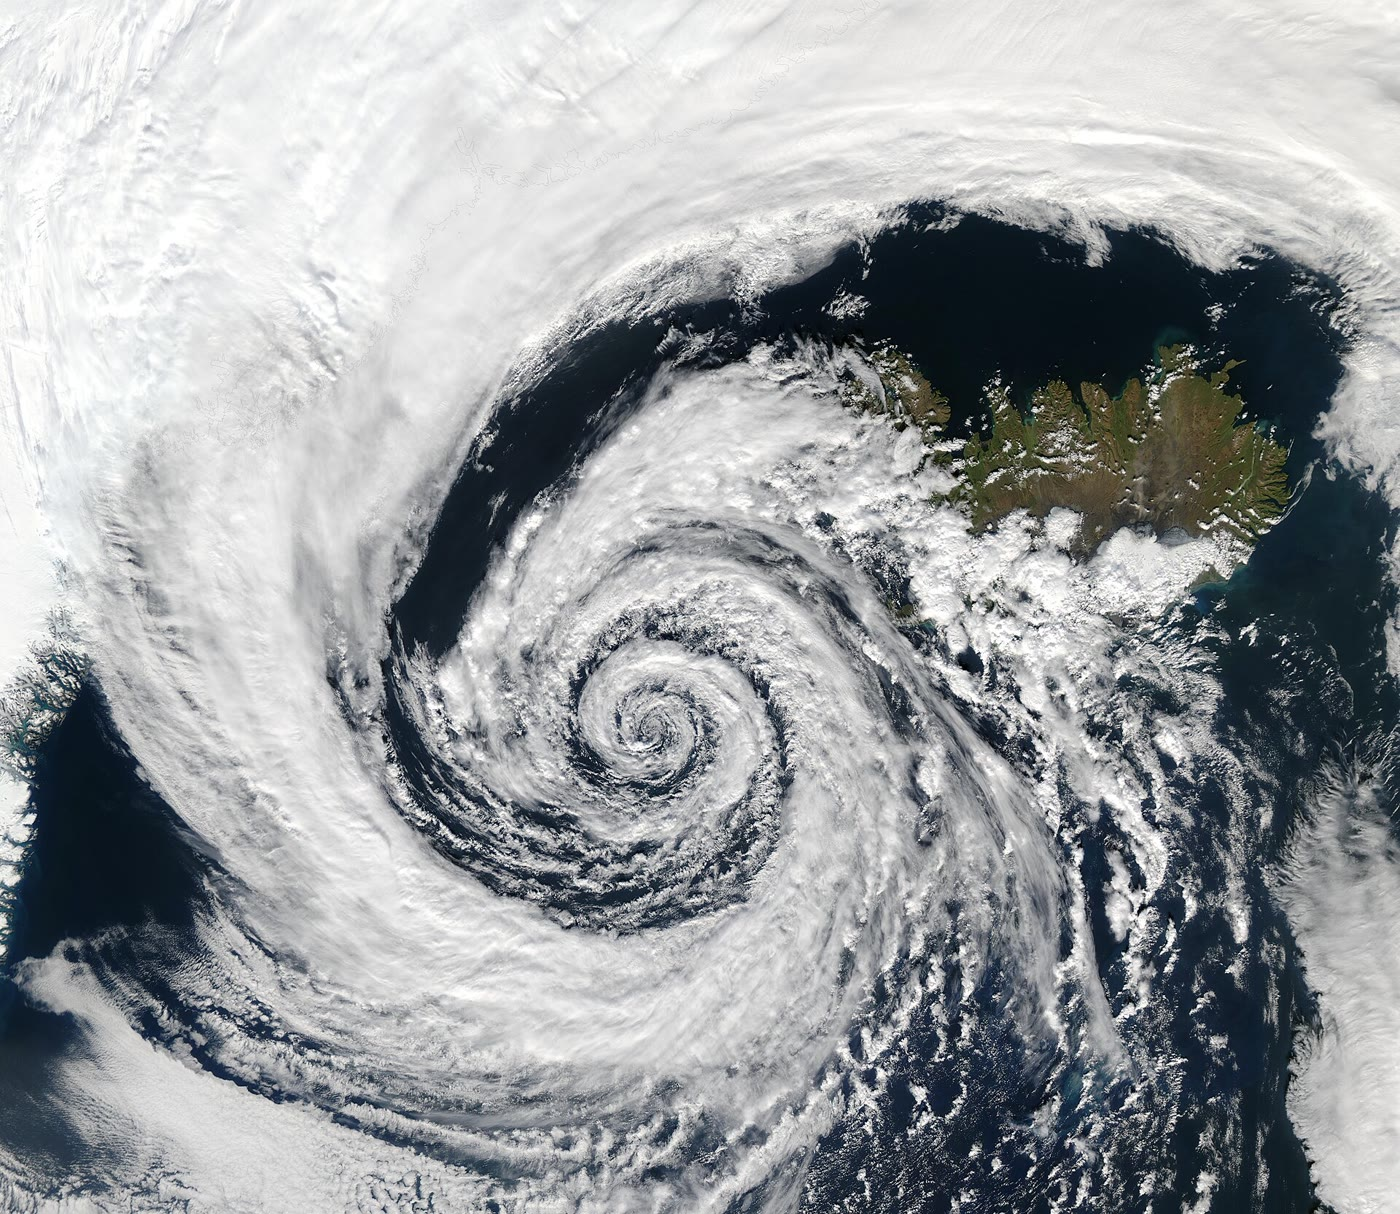
\includegraphics[width=\linewidth]{images/book5/b3-iceland-low.jpg}
\end{minipage}

\par\smallskip{\small Links, de Eady-groeisnelheid als functie van de golflengte voor de
januari \omterm{def:b3:atmospheric-dynamics:eddy}{zonaal gemiddelde} windschering op \ang{45}~NB (NCEP--NCAR Reanalysis~1,
1991--2020), de gemiddelde troposferische gelaagdheid en $H = \qty{11}{km}$:
geen groei onder \qty{3200}{km}, snelste groei nabij \qty{4700}{km}. Rechts, een
depressie in haar volwassen stadium voor de zuidwestkust van IJsland, 4
september 2003, haar wolken gewonden in een tegenwijzerszinnige spiraal rond het
lage drukcentrum (NASA/GSFC, MODIS Rapid Response Team, publiek
domein).}\label{fig:b3:atmospheric-dynamics:eady}
\end{omfigure}
% ledger: data:b5-ncep-uwnd, nasa:grc-atmos, photo:b3-iceland-low

De extratropische cycloon uit Boek~4 is het oppervlaktegezicht van een
groeiende barokliene golf: zijn warme sector voert warme lucht naar de pool en
omhoog, de koude lucht erachter schuift naar de evenaar en omlaag, en de trog
op grotere hoogte kantelt naar het westen met de hoogte, zoals de vrijkomst van \omterm{def:b3:atmospheric-dynamics:ape}{beschikbare potentiële
energie} vereist.

\section{De algemene circulatie}\label{sec:b3:atmospheric-dynamics:general-circulation}

De algemene circulatie wordt beschreven door te middelen langs breedtecirkels,
en wat het gemiddelde weglaat is even belangrijk als wat het behoudt.

\begin{definition}[Zonaal gemiddelde en wervels]\label{def:b3:atmospheric-dynamics:eddy}
Het \emph{zonaal gemiddelde}\index{zonaal gemiddelde} van een grootheid $A$ is het gemiddelde
langs een breedtecirkel op vaste hoogte of druk, $[A] =
(1/2\pi)\int_0^{2\pi} A\,\mathrm d\lambda$. De afwijking $A^* = A - [A]$
is haar wervelbijdrage; een \emph{wervel}\index{wervel (atmosferisch)} van de
atmosfeer is elke afwijking van de stroming ten opzichte van haar zonaal gemiddelde:
reizende golven, stationaire golven, cyclonen en anticyclonen.
\end{definition}

Het \omterm{def:b3:atmospheric-dynamics:eddy}{zonaal gemiddelde} van een product splitst zich in twee: $[vT] = [v][T] + [v^*T^*]$. De
eerste term is het transport door de gemiddelde meridionale circulatie, de cellen
van Boek~3; de tweede het transport door de \omterm{def:b3:atmospheric-dynamics:eddy}{wervels}. In de
middelste breedten is de gemiddelde meridionale wind zwak en domineert de wervelterm:
naar de pool bewegende lucht is warmer dan naar de evenaar bewegende lucht op
dezelfde breedte, zoals in onderstaande figuur, en $[v^*T^*] > 0$. De \omterm{def:b3:atmospheric-dynamics:eddy}{wervels} voeren
ook westelijk impulsmoment, $[u^*v^*]$, van de subtropen naar de breedten
van de straalstroom, waardoor de straalstroom en de westenwinden aan de grond
tegen wrijving in stand blijven. De Ferrelcel uit Boek~3 is de gemiddelde
meridionale circulatie die dit werveltransport afdwingt.

\begin{omfigure}
\begin{tikzpicture}[>=stealth, font=\small, declare function={s(\x)=0.9*sin(\x r); t(\x)=0.9*sin((\x+1.0) r);}]
\draw[thick, black, domain=0:12.566, samples=120] plot (\x, {s(\x)});
\draw[omThm, thick, densely dashed, domain=0:12.566, samples=120] plot (\x, {t(\x)-0.15});
\foreach \x in {0.3, 6.58} {\draw[->, omThm, very thick] (\x,-1.1) -- (\x,1.15)
  node[above, font=\scriptsize] {warm};}
\foreach \x in {3.45, 9.73} {\draw[->, omDef, very thick] (\x,1.1) -- (\x,-1.15)
  node[below, font=\scriptsize] {koud};}
\node[font=\scriptsize, anchor=west] at (12.7,{s(12.566)}) {stroomlijn};
\node[font=\scriptsize, anchor=west, omThm] at (12.7,{t(12.566)-0.15}) {isotherm};
\draw[->] (-1.6,-1.1) -- (-0.6,-1.1) node[below, font=\scriptsize] {oost};
\draw[->] (-1.6,-1.1) -- (-1.6,-0.1) node[above, font=\scriptsize] {noord};
\node[font=\scriptsize] at (6.3,-1.95) {koude lucht naar het noorden, warme naar het zuiden};
\end{tikzpicture}

\par\smallskip{\small Een groeiende barokliene golf in bovenaanzicht (schematisch,
Noordelijk Halfrond, westelijke stroming). De isotherm (gestippeld) loopt
een kwart golflengte of minder achter op de stroomlijn, zodat de lucht die naar het noorden beweegt (rode
pijlen) is warmer dan de lucht die naar het zuiden beweegt op dezelfde breedte (blauw):
de golf voert warmte naar de pool, $[v^*T^*] >
0$.}\label{fig:b3:atmospheric-dynamics:heatflux}
\end{omfigure}

In de tropen zijn de \omterm{def:b3:atmospheric-dynamics:eddy}{wervels} zwak en voert de gemiddelde circulatie warmte
naar de pool, de Hadleycel. In Boek~3 werd vastgesteld dat lucht die vanaf
de evenaar in rust vertrekt en haar impulsmoment behoudt, zou met honderden
meters per seconde waaien op \ang{40}, en liet open waarom de cel bij
\ang{30} eindigt. Een eenvoudig model geeft het antwoord.

\begin{definition}[Atmosferisch impulsmoment; Held--Hou-model]\label{def:b3:atmospheric-dynamics:held-hou}
Het \emph{atmosferisch impulsmoment}\index{atmosferisch impulsmoment}
per massa-eenheid om de aardas is $M = (\Omega a\cos\varphi +
u)\,a\cos\varphi$, voor een naar het oosten waaiende wind $u$ op breedte $\varphi$. Het
\emph{Held--Hou-model}\index{Held--Hou-model} van de Hadleycel is een
axisymmetrische, stationaire circulatie van een droge Boussinesq-atmosfeer met diepte
$H$, verwarmd door relaxatie naar een potentiële temperatuur van stralingsevenwicht
$\theta_E/\theta_0 = 1 + \Delta/3 - \Delta\sin^2\varphi$; de bovenste tak
behoudt $M$, de onderste tak heeft verwaarloosbare wind, en de
stroming is in thermische-windbalans.
\end{definition}

\begin{theorem}[Omvang van de Hadleycel]\label{thm:b3:atmospheric-dynamics:held-hou}
In de kleine-hoekbenadering bereikt de Held--Hou-cel de breedte
\[
\varphi_H = \left(\frac{5\,gH\Delta}{3\,\Omega^2a^2}\right)^{1/2}
\]
op elk halfrond, en de wind van zijn bovenste tak is $u_M = \Omega
a\varphi^2$.
\end{theorem}

\begin{proof}
Bij kleine $\varphi$ geldt $\cos\varphi \approx 1$, en lucht die de evenaar verlaat,
in rust met $M = \Omega a^2$ heeft de wind $u_M = \Omega a(1 - \cos^2\varphi)/\cos\varphi
\approx \Omega a\varphi^2$. Met $f \approx 2\Omega\varphi$, $y = a\varphi$,
geen wind aan de grond en de \omterm{thm:b3:gfd-foundations:thermal-wind}{thermische wind} in zijn Boussinesq-vorm over de
diepte $H$, $2\Omega\varphi\,u_M/H = -(g/a\theta_0)\,\partial\theta_M/
\partial\varphi$, waarbij $\theta_M$ het verticale gemiddelde van $\theta$ in de
cel is. Dan geldt $\partial(\theta_M/\theta_0)/\partial\varphi = -2\Omega^2a^2
\varphi^3/(gH)$ en $\theta_M/\theta_0 = A - K\varphi^4$, $K = \Omega^2a^2/
(2gH)$. Binnen de cel verplaatst de circulatie warmte, maar creëert noch
vernietigt ze, dus heeft de cel dezelfde gemiddelde temperatuur als het
stralingsevenwicht: $\int_0^{\varphi_H}\theta_M\,\mathrm d\varphi = \int_0^{\varphi_H}
\theta_E\,\mathrm d\varphi$. Aan de rand is de temperatuur continu:
$\theta_M(\varphi_H) = \theta_E(\varphi_H)$. Met $\theta_E/\theta_0 \approx
B - \Delta\varphi^2$, $B = 1 + \Delta/3$, geeft de eerste voorwaarde $A - B =
K\varphi_H^4/5 - \Delta\varphi_H^2/3$, de tweede $A - B = K\varphi_H^4 -
\Delta\varphi_H^2$. Aftrekken levert $(4/5)K\varphi_H^4 = (2/3)\Delta
\varphi_H^2$, dus $\varphi_H^2 = 5\Delta/(6K) = 5gH\Delta/(3\Omega^2a^2)$.
\end{proof}

De cel eindigt waar de temperatuur die het behoud van impulsmoment
oplegt, samenkomt met stralingsevenwicht; verder zou de atmosfeer kouder
moeten zijn dan straling haar maakt. Het model heeft twee parameters die
niet rechtstreeks worden waargenomen. Voor $H = \qty{15}{km}$ en $\Delta$ tussen $1/6$ en
$1/3$, gekozen ter illustratie, ligt $\varphi_H$ tussen \ang{25} en \ang{35}. De
waargenomen cellen, afgelezen uit de \omterm{def:b3:atmospheric-dynamics:eddy}{zonaal gemiddelde} meridionale wind, eindigen op
\ang{33.3}~NB en \ang{32.5}~ZB in het jaargemiddelde, en de wintercellen,
de sterke, op \ang{30.8}~NB in december--februari en \ang{29.1}~ZB in
juni--augustus. De schaling is het punt: een cel die breder wordt bij een
diepere troposfeer en een sterker verwarmingscontrast, en smaller wordt op een
sneller roterende planeet. De bovenwind van het model, $u_M =
\qty{88}{m/s}$ aan zijn rand voor $\Delta = 1/6$, is twee keer de waargenomen straalstroom:
de \omterm{def:b3:atmospheric-dynamics:eddy}{wervels} nemen het overschot weg.
% ledger: geod5:grs80-defining, earth:Rmean, data:b5-ncep-vwnd (values in figdata/bachelor-3/held_hou.py)

\begin{omfigure}
\begin{tikzpicture}
\begin{groupplot}[group style={group size=2 by 1, horizontal sep=1.7cm},
  width=0.48\linewidth, height=0.44\linewidth, tick label style={font=\scriptsize},
  label style={font=\small}, legend style={font=\scriptsize, draw=none, fill=none}]
\nextgroupplot[xlabel={breedtegraad (\unit{\degree})}, ylabel={$100\,(\theta/\theta_0 - 1)$},
  xmin=0, xmax=60, ymin=-30, ymax=15, legend pos=south west, legend cell align=left,
  title={\small $\Delta = 1/3$, $H = \qty{15}{km}$}]
% computed in figdata/bachelor-3/held_hou.py
\addplot[omDef, thick] table[x=phi, y=thE] {figdata/out/bachelor-3-held_hou-theta-3.dat};
\addplot[omThm, thick, unbounded coords=jump] table[x=phi, y=thM] {figdata/out/bachelor-3-held_hou-theta-3.dat};
\addplot[black!50, densely dashed, forget plot] coordinates {(35.26,-30) (35.26,15)};
\node[font=\scriptsize, anchor=south west] at (axis cs:35.6,7) {$\varphi_H$};
\legend{$\theta_E$, $\theta_M$}
\nextgroupplot[xlabel={breedtegraad (\unit{\degree})}, ylabel={$\psi$ op \qty{500}{hPa} ($10^{10}$\,\unit{kg/s})},
  xmin=-60, xmax=60, ymin=-25, ymax=25, xtick={-60,-30,0,30,60}, legend pos=south west,
  legend cell align=left]
\addplot[black!50, thin, domain=-60:60, samples=2, forget plot] {0};
\addplot[black, thick] table[x=lat, y=ann] {figdata/out/bachelor-3-held_hou-psi.dat};
\addplot[omDef, thick] table[x=lat, y=djf] {figdata/out/bachelor-3-held_hou-psi.dat};
\addplot[omThm, thick] table[x=lat, y=jja] {figdata/out/bachelor-3-held_hou-psi.dat};
\legend{jaar, dec--feb, jun--aug}
\end{groupplot}
\end{tikzpicture}

\par\smallskip{\small Links, de Held--Hou-constructie: de
impulsmoment-behoudende temperatuur van de cel (rood) ontmoet het
stralingsevenwicht (blauw) bij $\varphi_H = \ang{35}$, met gelijke oppervlakten tussen de
curven binnen de cel. Rechts, de gemiddelde meridionale massastroomfunctie op
\qty{500}{hPa} uit de \omterm{def:b3:atmospheric-dynamics:eddy}{zonaal gemiddelde} meridionale wind (NCEP--NCAR
Reanalysis~1, 1991--2020; positief waar de lucht boven \qty{500}{hPa}
noordwaarts beweegt): de sterke
winterhalfrond-cel reikt over de evenaar, en de cellen eindigen bij
\ang{30}.}\label{fig:b3:atmospheric-dynamics:held-hou}
\end{omfigure}
% ledger: data:b5-ncep-vwnd

\begin{history}[Van lange golven tot de eerste berekende verwachting]
In 1939 stelden C.-G.~Rossby en zijn medewerkers, in het \emph{Journal of Marine
Research}, zich ten doel om verschillende schijnbaar onafhankelijke verschijnselen
van het weer vanuit één gezichtspunt te duiden. Geïnspireerd door weerpatronen die
stroomopwaarts bewegen tegen de heersende westelijke stroming in, formuleerde Rossby
een gelineariseerde theorie waarin grootschalige verstoringen ten opzichte van de wind de neiging hebben westwaarts te bewegen
en kleinere oostwaarts, ten opzichte van de wind: de golven en de
$\beta$-vlak van dit hoofdstuk. Elf jaar later namen J.~G.~Charney,
R.~Fjørtoft en J.~von~Neumann de \omterm{thm:b3:atmospheric-dynamics:bve}{barotrope vorticiteitsvergelijking}
numeriek door op de elektronische computer ENIAC: vier verwachtingen van 24~uur op
het \qty{500}{mb}-niveau, op een rooster van \qty{736}{km}, 8 graden lengte
bij \ang{45}. De berekening van elke verwachting duurde ongeveer 24~uur: ze
waren, zoals zij schreven, net in staat het tempo van het weer bij te houden.
\end{history}
% ledger: rossby39:paper, jmr20:commentary, charney50:eniac

\section{Oefeningen}

\begin{exercise}[$\star$]\label{exo:b3:atmospheric-dynamics:1}
(a)~Bereken de \omterm{def:b3:atmospheric-dynamics:vorticity-kinds}{relatieve vorticiteit} van een \omterm{def:b3:atmospheric-dynamics:eddy}{wervel} in starre rotatie die
eenmaal per dag draait. (b)~Bereken de \omterm{def:b3:atmospheric-dynamics:vorticity-kinds}{planetaire vorticiteit} op \ang{30}~NB en \ang{60}~NB
($\Omega = \qty{7.292e-5}{rad/s}$) en vergelijk.
\end{exercise}

\begin{exercise}[$\star$]\label{exo:b3:atmospheric-dynamics:2}
Een luchtpakketje zonder \omterm{def:b3:atmospheric-dynamics:vorticity-kinds}{relatieve vorticiteit} op \ang{30}~NB beweegt naar \ang{40}~NB in een
stroming zonder divergentie. Bereken de \omterm{def:b3:atmospheric-dynamics:vorticity-kinds}{relatieve vorticiteit} daar. Is die
cyclonaal of anticyclonaal?
\end{exercise}

\begin{exercise}[$\star$]\label{exo:b3:atmospheric-dynamics:3}
Op \ang{45}~NB, zonder gemiddelde wind, bereken de fasesnelheid van een Rossby-golf
met golflengte \qty{5000}{km} en $l = 0$. In welke richting beweegt hij?
\end{exercise}

\begin{exercise}[$\star$]\label{exo:b3:atmospheric-dynamics:4}
Op \ang{60}~NB in een westenwind van \qty{10}{m/s}, bereken $\beta$, de
stationaire golflengte en het aantal stationaire golven rond de
breedtecirkel ($a = \qty{6371}{km}$).
\end{exercise}

\begin{exercise}[$\star\star$]\label{exo:b3:atmospheric-dynamics:5}
Een luchtkolom van \qty{10}{km} diep, zonder \omterm{def:b3:atmospheric-dynamics:vorticity-kinds}{relatieve vorticiteit} op \ang{45}
NB, passeert een bergketen die haar tot \qty{8}{km} samenperst, daarna een bekken
waar ze \qty{12}{km} diep is. Neem aan dat ze dicht bij \ang{45}~NB blijft; bereken haar
\omterm{def:b3:atmospheric-dynamics:vorticity-kinds}{relatieve vorticiteit} boven de keten en boven het bekken. Waar zullen
depressies zich waarschijnlijk vormen?
\end{exercise}

\begin{exercise}[$\star\star$]\label{exo:b3:atmospheric-dynamics:6}
Voor de golf met vijf toppen rond de breedtecirkel op \ang{45}~NB ($l = 0$) in een
westenwind van \qty{15}{m/s}, bereken de fasesnelheid en de groepssnelheid.
Hoe lang doet de energie van de golf erover om \qty{5000}{km} oostwaarts te reizen, en
hoe lang het patroon erover doet?
\end{exercise}

\begin{exercise}[$\star\star$]\label{exo:b3:atmospheric-dynamics:7}
Op \ang{45}~NB in een westenwind van \qty{15}{m/s} is een golf opgesloten tussen
breedtegraden, zodat $l = \pi/(\qty{6000}{km})$. (a)~Bereken de stationaire
zonaal golfgetal en golflengte. (b)~Toon aan dat er geen stationaire golf bestaat voor
$l = \pi/(\qty{3000}{km})$.
\end{exercise}

\begin{exercise}[$\star\star$]\label{exo:b3:atmospheric-dynamics:8}
In een \omterm{def:b3:atmospheric-dynamics:eady}{Eady-model} op \ang{45}~NB, $\Lambda = \qty{2e-3}{s^{-1}}$, $N =
\qty{0.012}{s^{-1}}$ en $H = \qty{10}{km}$. Bereken $L_d$, de groeisnelheid
en $e$-vouwtijd van de snelst groeiende verstoring, en de
golflengte daarvan.
\end{exercise}

\begin{exercise}[$\star\star$]\label{exo:b3:atmospheric-dynamics:9}
Langs een breedtecirkel is de meridionale wervelwind $v^* = V\cos kx$ en de
wervelcomponent van de temperatuur $T^* = T_0\cos(kx - \delta)$, met $V = \qty{10}{m/s}$ en
$T_0 = \qty{5}{K}$. Bereken $[v^*T^*]$ voor $\delta = 0$, \ang{60} en
\ang{90}, en de bijbehorende warmteflux $\rho c_p[v^*T^*]$ per
\unit{kg/m^3} lucht ($c_p = \qty{1004}{J.kg^{-1}.K^{-1}}$). Welke
opstelling transporteert geen warmte?
\end{exercise}

\begin{exercise}[$\star\star\star$]\label{exo:b3:atmospheric-dynamics:10}
Leid, uitgaande van de \omterm{thm:b3:atmospheric-dynamics:bve}{barotrope vorticiteitsvergelijking}, de \omterm{thm:b3:atmospheric-dynamics:rossby}{dispersierelatie
van Rossby-golven} in een uniforme westenwind af, en toon aan dat ten opzichte van
de lucht elke Rossby-golf zich westwaarts beweegt.
\end{exercise}

\begin{exercise}[$\star\star\star$]\label{exo:b3:atmospheric-dynamics:11}
Neem in het \omterm{def:b3:atmospheric-dynamics:held-hou}{Held--Hou-model} $H = \qty{12}{km}$ en $\Delta = 1/4$. Bereken
$\varphi_H$, de windsnelheid $u_M$ in de kleine-hoekbenadering aan de rand en de
exacte impulsmomentwind daar, en vergelijk die met de subtropische straalstroom van
\qty{44}{m/s} van het \omterm{def:b3:atmospheric-dynamics:eddy}{zonaal gemiddelde} van januari.
\end{exercise}

\begin{exercise}[$\star\star\star$]\label{exo:b3:atmospheric-dynamics:12}
Twee luchtlagen verschillen in potentiële temperatuur met \qty{10}{K} bij
\qty{300}{K}; hun grensvlak helt omhoog richting de pool met helling $s$
over een band van \qty{4000}{km} breed, en $\rho = \qty{0.7}{kg/m^3}$. (a)~Toon aan
dat het afvlakken van het grensvlak $\rho g' s^2L^2/24$ per oppervlakte-eenheid vrijmaakt,
$g' = g\,\Delta\theta/\theta$. (b)~Bereken die voor $s = 10^{-3}$ en
$2\times10^{-3}$ en vergelijk die met de kinetische energie van een wind van
\qty{15}{m/s} door \qty{10}{km} van dezelfde lucht.
\end{exercise}
% ledger: geod5:grs80-defining, earth:Rmean, data:b5-ncep-uwnd

\section{Probleem: De golf die stilstond}

\begin{problem}[{Weekendprobleem --- vorticiteit, Rossby-golven en de
groei van een barokliene golf op \ang{45} NB}]
\label{pb:b3:atmospheric-dynamics:1}
Een westenwind van \qty{15}{m/s} trekt over de middelbare breedten van een
verzonnen continent, langs \ang{45} NB. Neem $\Omega =
\qty{7.292115e-5}{rad/s}$, $a = \qty{6371}{km}$ en $g = \qty{9.81}{m/s^2}$.
Alle waarden van de stroming zijn verzonnen.

\medskip\noindent\textbf{Deel I --- Een verplaatst luchtpakketje.}
\begin{enumerate}
\item Een luchtpakketje zonder \omterm{def:b3:atmospheric-dynamics:vorticity-kinds}{relatieve vorticiteit} op \ang{45} NB wordt naar
  \ang{50} NB geduwd. Bereken $f$ op beide breedtegraden en de \omterm{def:b3:atmospheric-dynamics:vorticity-kinds}{relatieve vorticiteit} op
  \ang{50} NB, als de stroming geen divergentie heeft.
\item Langs welke krommingsstraal draait het, bewegend met \qty{15}{m/s}
  (neem $\zeta = -V/R$, alles afkomstig van de kromming)? In welke richting draait het?
\item Als de kolom onderweg ook krimpt van \qty{10.0}{km} tot \qty{9.5}{km},
  wat is dan de \omterm{def:b3:atmospheric-dynamics:vorticity-kinds}{relatieve vorticiteit} op \ang{50} NB?
\item Geduwd naar \ang{40} NB in plaats daarvan, zonder divergentie, welke \omterm{def:b3:atmospheric-dynamics:vorticity-kinds}{relatieve
  vorticiteit} krijgt het dan? Verklaar waarom een uit zijn breedte verplaatst luchtpakketje
  rond die breedte oscilleert.
\end{enumerate}

\medskip\noindent\textbf{Deel II --- Lopende golven.}
\begin{enumerate}[resume]
\item Bereken $\beta$ op \ang{45} NB en de lengte van de breedtecirkel.
\item Voor $n = 3$ tot en met 8 golven rond de cirkel ($l = 0$), bereken de
  golflengte, de fasesnelheid en de groepssnelheid in de westenwind van
  \qty{15}{m/s}.
\item Welke golven bewegen westwaarts en welke oostwaarts? Hoeveel dagen
  heeft de golf $n = 5$ nodig om \qty{1000}{km} te verplaatsen?
\item Een rug over het westen van het continent versterkt zich. Waar en na hoeveel
  tijd zal het effect van de golf $n = 6$ \qty{5000}{km}
  stroomafwaarts bereiken?
\end{enumerate}

\medskip\noindent\textbf{Deel III --- De golf die stilstond.}
\begin{enumerate}[resume]
\item Bereken de stationaire golflengte en het stationaire golfgetal op
  \ang{45} NB.
\item Bereken het stationaire golfgetal voor westenwinden van 10 en
  \qty{20}{m/s}. Wat gebeurt er met de stationaire golven wanneer de westenwinden
  in de winter versterken?
\item Bereken het stationaire golfgetal op \ang{35} NB en \ang{55} NB in de
  westenwind van \qty{15}{m/s}.
\item De westelijke bergen van het continent steken \qty{2}{km} op in een
  troposfeer van \qty{10}{km} diep. Bereken de \omterm{def:b3:atmospheric-dynamics:vorticity-kinds}{relatieve vorticiteit} van een kolom
  die de bergen passeert zonder van breedte te veranderen. Waarom forceren bergen
  stationaire golven?
\item Waarom staat het golfpatroon dat de bergen forceren alleen stil
  wanneer de golflengte dicht bij $\lambda_s$ ligt?
\end{enumerate}

\medskip\noindent\textbf{Deel IV --- Een storm groeit.}
\begin{enumerate}[resume]
\item De westenwind neemt van de grond tot \qty{10}{km} toe met
  \qty{25}{m/s}. Bereken de windschering $\Lambda$ en de naar de pool gerichte
  temperatuurgradiënt die daaruit volgt via de \omterm{thm:b3:gfd-foundations:thermal-wind}{thermische wind} bij een gemiddelde
  temperatuur van \qty{250}{K}.
\item Bereken met $N = \qty{0.011}{s^{-1}}$ het Richardson-getal
  $N^2/\Lambda^2$. Is de stroming instabiel voor kleinschalige schuifturbulentie?
\item Bereken de Rossby-straal $L_d$ voor $H = \qty{10}{km}$.
\item Bereken de golflengte van de snelst groeiende Eady-verstoring en
  het aantal van zulke golven rond de breedtecirkel.
\item Bereken de kortste golflengte die groeit.
\item Bereken de groeisnelheid $\sigma_{\max}$.
\item Met welke factor groeit de verstoring in drie dagen?
\item Vergelijk de golflengte van de groeiende storm met de stationaire
  golflengte van Deel~III: welke is langer, en wat betekent dat voor de
  beweging van de stormen ten opzichte van de stationaire golven?
\item In welke richting kantelt de trog van de groeiende golf met de hoogte, en
  waarom moet dat?
\item Geef de $e$-vouwtijd van de snelst groeiende Eady-verstoring.
\end{enumerate}
\end{problem}
% ledger: geod5:grs80-defining, earth:Rmean
